\emph{Knowledge graphs} (KGs) power search engines, question-answering systems and social networks. They are especially useful to manage dynamic, diverse data and have drawn significant attention from industry and academia in recent years~\cite{}. Today, many big tech companies, such as Amazaon~\cite{AmazonKG}, Facebook~\cite{}, Google~\cite{} and Microsoft~\cite{MicrosoftKG} run their own enterprise knowledge graphs. But, although the term "Knowledge Graph" became popular only in 2012 when Google announced its equally named system~\cite{}, the concept behind it is much older and even the term itself has been used back in the 70s~\cite{}.

Since then many definitions for knowledge graphs have been given, often contradicting each other, but in general they all describe knowledge graphs as directed graphs whose nodes and edges represent objects and their relationships to each other. In this work, a knowledge graph $G$ is formally defined as a set of known facts, which are a subset of all facts that could theoretically be constructed between the set of entities $E$ and the set of relations $R$:

\[
    G \subseteq E \times R \times E
\]

Due to their mathematical structure, facts are also referred to as \emph{triples}. A fact $(head, rel, tail)$ consists of a \emph{head} entity, a \emph{tail} entity and a relation between the two. Relations are usually not symetrical and therefore represented by directed edges. Figure~\ref{fig:1_introduction/knowledge_graph} shows an example knowledge graph as it could be used in a social network. It stores knowledge about concrete objects as well as general concepts, such as the fact $(Ed, has~gender, male)$. Symmetrical relations, such as "married to" are represented by two directed edges.

\begin{figure}[t]
    \centering
    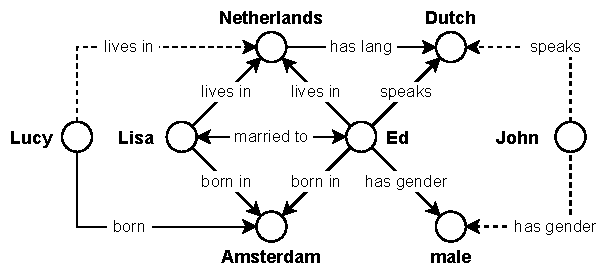
\includegraphics[]{1_introduction/knowledge_graph}
    \caption{Example Knowledge Graph. Some facts missing}
    \label{fig:1_introduction/knowledge_graph}
\end{figure}

Besides displaying known facts using solid lines, Figure~\ref{figure:example_knowledge_graph} also shows dotted lines which indicate facts that hold true in reality but which are missing from the graph, like the fact $(Lucy, lives in, Netherlands)$. In fact, real-world knowledge graphs are often rather incomplete for several reasons: Firstly, it is difficult to manually create and update a large graph in the first place, and secondly, facts are sometimes deliberately left out if they can be derived from other facts. An example for the latter would be the transitive relation "lies in": Given a graph that stores $(Paris, lies in, France)$ and $(France, lies in Europe)$, it can be derived that Paris lies in Europe. This circumstance, that given facts can be relied on, but missing facts are not automatically false, but rather unknown, is known as \emph{open-world scenario}~\cite{}. If, instead, missing facts were actually false, the \emph{closed-world assumption} would hold instead.

When looking close at Figure~\ref{fig:1_introduction/knowledge_graph}, patterns can be found in the graph structure. For example, two out of three people born in Amsterdam also speak Dutch. One could therefore correctly assume that this is also true for the third entity Lucy. Furthermore, the fact that person A is married to person B also seems to imply that person B is married to person A. Two fundamentally different approaches to capturing these patterns are (1) searching for logical rules that generalize individual cases or (2) projecting the graph into a vector space, also known as \emph{embedding}, in which the patterns can easily be registered by machines.

Most state-of-the-art models follow the embedding approach, as it proved effective and efficient for a wide range of tasks including image \cite{}, natural language \cite{} and graph processing \cite{}. Embedding-based approaches are also called latent, because the exact structure of their embedding space is incomprehensible, or latent, to humans. In contrast, classical rule-based approaches are denoted as symbolic and bring the advantage that their rules are meaningful to humans - other from a 300-dimensional vector in an embedding space. In their paper on the AnyBURL rule miner \cite{}, Melicke et al. that rule-based models are capable to perform equally well to embedding-based approaches and demand further research on rule-based approaches.

Following that suggestion, this work builds a rule-based knowledge graph completion model on top of AnyBURL and combines it with a text-based model, forming the \emph{Power} ensemble model, which stands for "\textbf{P}robabilistic \textbf{o}pen-\textbf{w}orld \textbf{e}xtension to \textbf{r}ule-based KGC". Besides improving the rule-based component's fact predictions by leveraging additional text information, the text-based component enables predictions for open-world entities for which no facts are given. One of the top aims for both rule-based and text-based prediction was explaining the models decision. Therefore, each predicted fact is given with a lists of the rules and sentences that led to it.

As an example, considering the entity Lucy in Figure~\ref{fig:1_introduction/knowledge_graph}, who is known to be born in Amsterdam, the Power model would suggest that she lives in the Netherlands and give the rule $(X, lives in, Netherlands) <= (X, born in, Amsterdam)$ with a confidence of 67\% as an explanation. If multiple rules predict the same fact, all rules with a confidence greater 50\% are given in sorted order. In parallel to the rule-based prediction, a text about Lucy, like "Lucy is from the Netherlands", might lead to a 90\% prediction of $(Lucy, lives~in, Netherlands)$ by the text-based component. When multiple texts are given, they are ordered by relevance, as well. For open-world entities like John, the rule-based component cannot apply any rules, so analyzing John's texts is the only way to possibly predict his knowledge of Dutch or the fact that he is male. Again, multile texts, like "John is Dutch" and "He is an actor", are sorted by relevance to explain to the user that the fact $(John, speaks, Dutch)$ was inferred due the first sentence while the prediction of $(John, has~gender, male)$ is primarily based on the second one.

In the following, Chapter~\ref{ch:2_related_work} explains some basics and terminology about rules, neural networks and metrics that are used throughout this thesis. Next, Chapter~\ref{ch:3_basics} gives an overview of the variety of ways to approach knowledge graph completion using embedding and rule-based models before Chapter~\ref{ch:4_approach} explains the Power model's implementation. Subsequently, Chapter~\ref{ch:5_experiments} presents the evaluation results as well as experiments on variations of the Power model and Chapter~\ref{ch:6_conclusion} concludes with a summary and suggestions for further research. Appendix~\ref{ch:a_appendix} contains tables and graphs that have been separated for readability.

The Python implementation of the Power model is available on GitHub~\cite{GitHubPower} under the MIT open-source license. Additionally, multiple other repositories provide the code for the experiments~\cite{}.
